\documentclass[aspectratio=169]{beamer}

\usetheme{boxes}
\useinnertheme{circles}

\definecolor{UC}{RGB}{0, 50, 98}
\definecolor{Beamer}{RGB}{51, 51, 178}
\definecolor{Hooker}{RGB}{73, 121, 107}
\definecolor{Triton}{RGB}{0, 106, 150}
\definecolor{Prussian}{RGB}{0, 49, 83}
\definecolor{Forest}{RGB}{101, 121, 48}
\definecolor{Metro}{RGB}{35, 55, 59}
\definecolor{Gamboge}{RGB}{228, 155, 15}
\definecolor{Devil}{RGB}{115, 39, 43}
\definecolor{Shade}{RGB}{250, 250, 250}
\definecolor{JPAL}{RGB}{227, 89, 37}
\definecolor{IPA}{RGB}{90, 128, 38}

\usecolortheme[named=Beamer]{structure}

% \setbeamercolor{background canvas}{bg=Shade}
\setbeamercolor{block title}{bg=Beamer!12}
\setbeamercolor{block body}{bg=Beamer!8}

\setbeamersize{text margin left=0.2in,text margin right=0.2in}

% \setbeamertemplate{footline} % To remove the footer line in all slides uncomment this line
\setbeamertemplate{footline}[page number] % To replace the footer line in all slides with a simple slide count uncomment this line
\setbeamertemplate{navigation symbols}{} % To remove the navigation symbols from the bottom of all slides uncomment this line
\setbeamertemplate{bibliography item}{}
\setbeamertemplate{caption}[numbered]

\setbeamertemplate{frametitle}{%
    \usebeamerfont{frametitle} \vspace{0.5em} \insertframetitle%
    \vphantom{g}% To avoid fluctuations per frame
    \vspace{0.5em} \hrule% Uncomment to see desired effect, without a full-width hrule
    \par\hspace*{-\dimexpr0.5\textwidth-0.5\textwidth}\rule[0.5\baselineskip]{\textwidth}{0.4pt}
    \par\vspace*{-\baselineskip}% <-- reduce vertical space after rule
}

\usepackage[T1]{fontenc}
\usepackage{inconsolata}
% \usepackage[sfdefault,light]{roboto}
\usepackage{cmbright}
% \usepackage[default]{lato}
\usepackage{amsmath, amssymb, amsthm, mathrsfs, bbm}
\usepackage{threeparttable, adjustbox, tabularx, booktabs}
\usepackage{appendixnumberbeamer}
\usepackage{hyperref}
\usepackage{pdflscape}
\usepackage{placeins}
\usepackage{caption}
\usepackage{graphicx}
\usepackage{listings}
\usepackage{color}
\usepackage{tfrupee}
\usepackage[backend=bibtex, style=authortitle, citestyle=authoryear-icomp, url=false]{biblatex}
\addbibresource{Lottery.bib}

\newcommand{\inv}[1]{#1^{-1}}
\newcommand{\iid}{\text{i.i.d.}}
\newcommand{\bmat}[1]{\begin{bmatrix} #1 \end{bmatrix}}
\newcommand{\asconv}{\xrightarrow{a.s.}}
\newcommand{\pconv}{\xrightarrow{p}}
\newcommand{\dconv}{\xrightarrow{d}}
\newcommand{\msconv}{\xrightarrow{m.s.}}
\newcommand{\liminfty}{\lim_{n \to \infty}}
\newcommand*\diff{\mathop{}\!\text{d}}
\newcommand{\lhood}{\mathcal{L}}
\newcommand{\var}{\text{Var}}
\newcommand{\ev}{\text{E}}
\renewcommand{\vec}[1]{\mathbf{#1}}
\newcommand{\specialcell}[2][c]{\begin{tabular}[#1]{@{}c@{}}#2\end{tabular}}

\newtheorem{prop}{Proposition}
\newtheorem{claim}{Claim}
\newtheorem{assume}{Assumption}
\newtheorem{define}{Definition}

\newenvironment{wideitemize}{\itemize\addtolength{\itemsep}{10pt}}{\enditemize}
\newenvironment{wideenumerate}{\enumerate\addtolength{\itemsep}{10pt}}{\endenumerate}

\let\oldforall\forall
\let\forall\undefined
\DeclareMathOperator{\forall}{\oldforall}
\DeclareMathOperator*{\argmax}{arg\,max}
\DeclareMathOperator*{\argmin}{arg\,min}

\lstset{
  basicstyle=\footnotesize\ttfamily,
  columns=fixed,
  fontadjust=true,
  basewidth=0.5em
}

\title{Using Lotteries to Encourage Savings: Experimental Evidence from Kenya}
\author[Abraham, Akbas, Ariely, Jang]{Justin Abraham\inst{1} \and Merve Akbas\inst{2} \and Dan Ariely\inst{2} \and Chaning Jang\inst{3}}
\institute{\inst{1} University of California, San Diego \and \inst{2} Duke University \and \inst{3} Busara Center for Behavioral Economics}
\date{\today}

\begin{document}

\begin{frame}
	\titlepage
\end{frame}

\begin{frame}{Savings as a Policy Objective}

	\begin{wideitemize}

		\item Access to savings is an important avenue toward economic development.

		\begin{wideitemize}

			\item Can be used to invest in productive assets when unable to borrow.

			\item Allows for some degree of consumption smoothing when insurance is incomplete. 

		\end{wideitemize}

		\item Only 22 percent of the world's poorest have an account at a financial institution \parencite{demirguc-kunt_global_2018}. Even less use them regularly.

		\item The prevalence of alternative strategies (livestock, cash under the mattress, informal groups) suggest a latent demand for saving.

		% Argue that there is room for policy intervention.

	\end{wideitemize}

\end{frame}

\begin{frame}{Savings as a Policy Objective}

	\begin{wideenumerate}

	% There are both supply and demand side constraints on financial inclusion. A large of the microdevelopment literature has been devoted to addressing financal constraints.

		% Initial and transaction costs can be prohibitive for the poor \parencite{karlan_savings_2014}. 

		\item Mobile technologies, bank expansions, lowering account requirements, etc. \parencite{jack_mobile_2011,dupas_challenges_2014,dupas_savings_2009,burgess_rural_2005}.

		% In Kenya, 80\% of adults have a banking account or mobile money but only 30\% actually use it to save \parencite{demirguc-kunt_global_2018}. So there are also constraints on the consumer side.
		
		\item Subsidy experiments estimate very low interest rate elasticities \parencite{karlan_price_2018,schaner_persistent_2018}.
		
		\item Financial literacy is low in developing countries and education interventions have mixed results \parencite{miller_can_2015}.
		
		\item Product design (default savings, commitment devices, reminders) targeted to problems of self-control/attentiveness have proven very cost-effective \parencite{ashraf_tying_2006,dupas_why_2013,somville_saving_2018}.

	\end{wideenumerate}

\end{frame}

\begin{frame}{Prize-Linked Savings}

	Prize-linked savings (PLS) provide stochastic returns to savings deposits (a lottery ticket for saving).

	\begin{wideitemize}
		\item There is policy interest in using this product as way to encourage saving \parencite{kearney_making_2010}.
		\item Has existed since the 17th century in England and common in many parts of the world \parencite{kearney_making_2010}.
		\item NS\&I Premium Bonds in the U.K. since 1956 and A-Million-A-Month in South Africa (defunct).
		\item Legal in the US since 2014.
	\end{wideitemize}

\end{frame}

\begin{frame}{Prize-Linked Savings}

	% From an (expected) revenue neutral perspective, 

	How might lotteries induce savings over regular interest-bearing accounts?

	% Related to an old question in economics about why people hold insurance and gamble.

	\begin{wideitemize}
		\item Thrill of playing \parencite{conlisk_utility_1993}.
		\item Large sums for purchasing durable goods when credit constrained/adjustment costs \parencite{herskowitz_gambling_2016}.
		\item Non-linear probability weighting \parencite{kahneman_advances_1992}.
		\item \textbf{Aversion to anticipated regret} can induce apparently risk-seeking behavior \parencite{loomes_regret_1982,bell_risk_1983,zeelenberg_consequences_1996}.
	\end{wideitemize}

\end{frame}

\begin{frame}{Research Questions}

	\begin{wideenumerate}

		\item Can prize-linked savings induce account usage in low income settings?
		\item How much of this effect can we attribute to a specific mechanism (regret aversion)?

	\end{wideenumerate}

\end{frame}

\begin{frame}{Overview}

	\begin{itemize}

		\item Provided a mobile savings account to 311 periurban residents of Nairobi, Kenya.
		\item Experimentally vary the incentive structure (fixed versus stochastic) and information structure.
		\item Observe account activity over a 60-day period.

		\begin{itemize}
			\item Test the effect of stochastic incentives
			\item Quantify the role of regret aversion
			\item Limited evidence on total savings, consumption, gambling
			\item Heterogeneous effects
		\end{itemize}

	\end{itemize}

\end{frame}

\begin{frame}{Related Literature}
	
	\begin{itemize}

		\item Do lottery-like incentives work? 
		
		\begin{itemize}
			\item In the lab, lotteries effectively increase the savings rate \parencite{atalay_savings_2014,filiz-ozbay_lottery_2015}. Evidence for non-linear probability weighting.
			\item In the field, works over many domains \parencite{dizon_leveraging_2016,gajic_cost-effectiveness_2011,brune_effect_2015,loibl_testing_2016,gertler_long-term_2017}.
		\end{itemize}

		\item Contributions

		\begin{itemize}
			\item Account usage as an outcome has been given little attention.
			\item A field experiment that quantifies the role of a specific channel.
			\item One of the few tests of regret aversion outside the lab.
		\end{itemize}

	\end{itemize}

\end{frame}

\begin{frame}{Study Setting}

	\begin{figure}[H]
		\centering
		\includegraphics[height=0.8\textheight]{kibera-tracks.jpg}
	\end{figure}

	% replace this with something personal

\end{frame}

\begin{frame}{Study Setting}

	Sample of 311 adults from Kibera and other settlements around Nairobi.

	\begin{wideitemize}
		\item Less than half of the sample consider themselves employed.
		\item Only 5\% receive regular income with an average of USD PPP 77 monthly.
		\item A little over half save regularly and most use ROSCAs.
		\item Average monthly savings amount to USD 23.
		\item 24\% report having gambling problems.
	\end{wideitemize}

	% https://qz.com/africa/1140842/gambling-addiction-is-on-the-rise-in-kenya-and-leaving-young-people-bankrupt-and-suicidal/

	% what do people save for?

\end{frame}

\begin{frame}{Mobile Savings}
	
	\begin{wideitemize}
		\item Respondents provided a mobile phone linked to a Sambaza account for 60 days.
		\item Make deposits by sending airtime free of charge.
		\item Respondents received daily SMS reporting balance.
		\item Lockbox savings; withdrawal allowed only on the 30th day.
		\item Principal returned after 60 days via M-Pesa.
	\end{wideitemize}

	% Everyone has a mobile phone, know how to use mobily money, cash out easily, high trust, in order to minimize the role of transaction costs/information/trust

	% limit transaction costs and setup costs

\end{frame}

\begin{frame}{Experiment}

	\begin{block}{Control ($N = 105$)}
		\begin{itemize}
		\item Certain 5\% match on daily deposits
		\item Daily balance and returns reported via SMS
		\end{itemize}
	\end{block}

	\begin{columns}[T]

		\begin{column}{0.48\textwidth}
			\begin{block}{PLS ($N = 103$)}
			\begin{itemize}
			\item Daily lottery equal in expectation to 5\% return
			\item Guarantees no losses
			\item Always gets a lottery ticket but redeemable if deposited
			\end{itemize}
			\end{block}
		\end{column}

		\begin{column}{0.48\textwidth}
			\begin{block}{PLS without feedback ($N = 103$)}
			\begin{itemize}
			\item Incentives identical to PLS
			\item Received a lottery ticket only if made a deposit that day
			\end{itemize}
			\end{block}
		\end{column}

	\end{columns}

\end{frame}

\begin{frame}{Data}

	\begin{wideenumerate}
		\item Subject demographics and preference elicitation from a lab session before the experiment.
		\item Detailed daily transaction data (deposits, withdrawals, balances).
		\item Savings by other means, self-reported gambling behavior, and program feedback from an endline questionnaire.
	\end{wideenumerate}

\end{frame}

\begin{frame}{Results}
	
	\centering \large I. What are the effects of prize-linked incentives on savings?

\end{frame}

\begin{frame}{Results -- Mobile Savings}

	\begin{table}[h]\centering \def\sym#1{\ifmmode^{#1}\else\(^{#1}\)\fi} \caption{Treatment effects -- Mobile savings} \label{tab:reg-mobile} \maxsizebox*{\textwidth}{\textheight}{ \begin{threeparttable} \begin{tabular}{l*{5}{c}} \toprule
          &\multicolumn{3}{c}{Effect estimates}&\multicolumn{2}{c}{Sample}\\\cmidrule(lr){2-4}\cmidrule(lr){5-6}
          &\multicolumn{1}{c}{(1)}&\multicolumn{1}{c}{(2)}&\multicolumn{1}{c}{(3)}&\multicolumn{1}{c}{(4)}&\multicolumn{1}{c}{(5)}\\
          &\multicolumn{1}{c}{Lottery}&\multicolumn{1}{c}{Regret}&\multicolumn{1}{c}{\specialcell{Regret-\\Lottery}}&\multicolumn{1}{c}{\specialcell{Control Mean\\(SD)}}&\multicolumn{1}{c}{Obs.}\\
\midrule
Total no. of deposits&4.59\sym{*}& & &    13.66&      311\\
          &   (2.52)& & &  (15.08)&         \\
No. of days saved&3.93\sym{*}& & &    11.78&      311\\
          &   (2.05)&    &    &  (12.93)&         \\
Total deposit amount&  -0.79   &     & &    14.87&      311\\
          &   (3.34)&    &    &  (24.48)&         \\
Total withdrawal amount&     0.53& &  &     1.07&      311\\
          &   (0.94)&    &   &   (4.53)&         \\
\bottomrule \end{tabular} \begin{tablenotes}[flushleft] \footnotesize \item \emph{Notes:} Columns 1--3 report OLS estimates of the treatment effect. Standard errors are in parentheses. Columns 4--5 report the mean and SD of the control group and the number observations, respectively. Observations are at the individual level. * denotes significance at 10 pct., ** at 5 pct., and *** at 1 pct. level. \end{tablenotes} \end{threeparttable} } \end{table}

% File produced by reg-main.do with /Users/justin/Repos/akiba-lottery-pub/data/clean/akiba_wide.dta on 12:30:21 10 Jun 2019 by user justin on Stata 13.1 with seed X53d8cd0fc43f462544a474abacbdd93d00044a8f

	% number of deposits but not savings; reflects the fact that knowing the results of the lottery hinges on the extensive margin

\end{frame}

\begin{frame}{Discussion -- Mobile Savings}

	\begin{wideitemize}
		\item Effects occur on the ``extensive margin''.
		\begin{wideitemize}
			\item Consistent with other studies of lottery incentives \parencite{brune_effect_2015,gertler_long-term_2017}.
			\item Can be rationalized as the subdivision of lotteries \parencite{samuelson_risk_1963}.
		\end{wideitemize}
		\item Null effect on savings amount likely due to liquidity constraints \parencite{loibl_testing_2016}.
		\item What does this tell us about potential mechanisms?
	\end{wideitemize}

\end{frame}

\begin{frame}{Results}
	
	\centering \large II. How much of the effect can be explained by regret aversion?

\end{frame}

\begin{frame}{A Theory of Regret}

	\begin{block}{Regret \parencite{zeelenberg_consequences_2004}}
	 ``...a negative, cognitively based emotion that we experience when realizing or imagining that our present situation would have been better, had we decided differently''
	\end{block}

\end{frame}

\begin{frame}{A Theory of Regret}

	\begin{itemize}

		\item Preferences depend on comparisons between outcomes of chosen and foregone prospects \parencite{bell_risk_1983,loomes_regret_1982}.

		\item Individuals experience regret after the resolution of prospects. Suppose state $i$ obtains, $f, g \in B$, and $f$ is chosen.

			\[ \Psi(f_i; g_i) = u(f_i) + \gamma R(u(f_i) - u(g_i)) \]

		\item $R$ is strictly increasing, decreasingly concave, and satisfies $R(0) = 0$.

		\item If individuals can anticipate regret/rejoicing then it affects ex ante behavior.

		\[ f \succsim g \leftrightarrow \sum_i p_{i} \cdot [\Psi(f_i; g_i) - \Psi(g_i; f_i)] \geq 0 \]

		% Difference from reference dependence/DA? I only make relative comparisons when I know that I will experience ex post regret. Disapointment is related to what might have been in an unrealized state in the same lottery but regret is about what have been in a foregone choice (regret is action-based).

		% When choices also affect resolution/experience of regret then it can affect behavior. 

		% Is it kinked? People postulate so but no quantification

	\end{itemize}
	
\end{frame}

\begin{frame}{Identifying Regret Aversion}

	\begin{wideitemize}

		\item Regret is not experienced (anticipated) if unchosen prospects are not resolved.

		\item This is the central test of regret aversion in the lab \parencite{filiz-ozbay_auctions_2007,zeelenberg_consequences_2004,zeelenberg_consequences_1996}.

		\item In our study, individuals in PLS treatments can experience regret only if they chose \textit{not} to save and learned about a winning ticket at the resolution of the daily lottery.

		% they cannot experience regret by choosing to enter the lottery because it cannot result in losses

		\item \textbf{Hypothesis}: More deposits with feedback than without.

	\end{wideitemize}

	% If lottery is more attractive in lottery then it implies R is negative here
	
\end{frame}

\begin{frame}{Results -- Regret Aversion}

	\begin{table}[htbp]\centering \def\sym#1{\ifmmode^{#1}\else\(^{#1}\)\fi} \caption{Treatment effects -- Mobile savings by respondent} \label{tab:reg-mobile} \maxsizebox*{\textwidth}{\textheight}{ \begin{threeparttable} \begin{tabular}{l*{8}{c}} \toprule
          &\multicolumn{3}{c}{No controls}&\multicolumn{3}{c}{With controls}&\multicolumn{2}{c}{Sample}\\\cmidrule(lr){2-4}\cmidrule(lr){5-7}\cmidrule(lr){8-9}
          &\multicolumn{1}{c}{(1)}&\multicolumn{1}{c}{(2)}&\multicolumn{1}{c}{(3)}&\multicolumn{1}{c}{(4)}&\multicolumn{1}{c}{(5)}&\multicolumn{1}{c}{(6)}&\multicolumn{1}{c}{(7)}&\multicolumn{1}{c}{(8)}\\
          &\multicolumn{1}{c}{Lottery}&\multicolumn{1}{c}{Regret}&\multicolumn{1}{c}{\specialcell{Difference\\\(p\)-value}}&\multicolumn{1}{c}{Lottery}&\multicolumn{1}{c}{Regret}&\multicolumn{1}{c}{\specialcell{Difference\\\(p\)-value}}&\multicolumn{1}{c}{\specialcell{Control Mean\\(SD)}}&\multicolumn{1}{c}{Obs.}\\
\midrule
Total no. of deposits&4.59$^{*}$&5.71$^{**}$&     0.69&4.53$^{*}$&4.76$^{**}$&     0.94&    13.66&      311\\
          &   (2.52)&   (2.45)&         &   (2.64)&   (2.42)&         &  (15.08)&         \\
          &   [0.20]&   [0.20]&         &   [0.30]&   [0.10]&         &         &         \\
No. of days saved&3.93$^{*}$&4.94$^{**}$&     0.66&3.56$^{*}$&4.19$^{**}$&     0.78&    11.78&      311\\
          &   (2.05)&   (2.08)&         &   (2.06)&   (2.05)&         &  (12.93)&         \\
          &   [0.20]&   [0.20]&         &   [0.40]&[0.00]$^{***}$&         &         &         \\
Avg. no. of deposits&    -0.02&    -0.01&     0.80&    -0.00&    -0.01&     0.81&     1.16&      275\\
          &   (0.04)&   (0.04)&         &   (0.04)&   (0.03)&         &   (0.29)&         \\
          &   [0.70]&   [0.90]&         &   [1.00]&   [1.00]&         &         &         \\
Log total deposit amt.&     0.04&     0.04&     0.98&     0.03&    -0.02&     0.84&     2.26&      311\\
          &   (0.22)&   (0.22)&         &   (0.22)&   (0.22)&         &   (1.63)&         \\
          &   [0.80]&   [0.90]&         &   [1.00]&   [1.00]&         &         &         \\
\bottomrule \end{tabular} \begin{tablenotes}[flushleft] \footnotesize \item \emph{Notes:} Columns 1 - 2 report OLS estimates of the treatment effect. Columns 4 - 5 reports the estimates controlling for baseline covariates. Columns 3 and 6 report the \(p\)-values for tests of the equality of the two treatment effects. Standard errors are in parentheses and FWER adjusted \(p\)-values are in brackets. Observations are at the individual level. * denotes significance at 10 pct., ** at 5 pct., and *** at 1 pct. level. Stars on the coefficient estimates reflect unadjusted \(p\)-values. \end{tablenotes} \end{threeparttable} } \end{table}

% File produced by reg-fwer.do with /Users/Justin/Repos/akiba-lottery-pub/data/clean/akiba_wide.dta on 12:19:39  2 Mar 2017 by user Justin on Stata 13.1 with seed X02be4b816237fe6e6a333726618fd6dd00043d82

\end{frame}

\begin{frame}{Results -- Regret aversion}

		\begin{figure}[ht]
		\centering
		\caption{Timing of deposits}
		\includegraphics[height=0.8\textheight]{../../figures/hist-deposits.pdf}
		\label{fig:hist-deposits}
		\caption*{\footnotesize \emph{Notes:} This figure plots the empirical distribution of timing of all deposits over the project period. Each bin spans 30 minutes with a height equal to the fraction of all deposits within each treatment group. A vertical line marks 8:00, when participants received the first SMS that summarized how much the participant saved the previous day, how much the participant earned through a matching contribution or winnings, and their total balance. An hour later, participants received a second SMS encouraging them to save that day. Participants in PLS received a new lottery ticket with the second message.}
		\end{figure}

		% people make deposits right when they get the lottery ticket and when results are announced

\end{frame}

% \begin{frame}{Results -- Regret Aversion}
	
	% Does experienced regret mediate anticipated regret?
	
	% \begin{table}[ht]\centering \def\sym#1{\ifmmode^{#1}\else\(^{#1}\)\fi} \caption{Regression of deposits on treatment and lottery results} \label{tab:reg-regretaversion} \maxsizebox*{\textwidth}{\textheight}{ \begin{threeparttable} \begin{tabular}{l*{2}{c}} \toprule
                &\multicolumn{1}{c}{Made a deposit}\\
\midrule
Winning ticket  &     0.02\sym{**} \\
                &   (0.01)         \\
\midrule
Adjusted \(R^{2}\)&    0.081         \\
Control mean    &     0.20         \\
Period 1 effect &                  \\
Observations    &     4473         \\
\bottomrule \end{tabular} \begin{tablenotes}[flushleft] \footnotesize \item \emph{Notes:} This table reports estimates of a regression of having saved at period \(t\) on winning the lottery at \(t\) conditional on being in the PLS group and not having saved at \(t=1\). The unit of observation is individual-by-period. Standard errors are in parentheses and clustered at the individual level. * denotes significance at 10 pct., ** at 5 pct., and *** at 1 pct. level. \end{tablenotes} \end{threeparttable} } \end{table}

% File produced by akiba-estimate.do with /Users/justin/Repos/akiba-lottery-pub/data/clean/akiba_long.dta on 11:37:03 19 Mar 2020 by user justin on Stata 13.1 with seed X440b457b8aac484a7d965296a0f1c153000412ab

	% 	Two effects: anticipation of multiple future resolutions, dependence on experienced

% 	1. Recently experienced regret can make anticipated regret more salient as in zeelenberg 
% 	2. Initial anticipation may be overconfident and people can learn (or other way)


% \end{frame}

\begin{frame}{Results}
	
	\centering \large How does the effect evolve over time?

\end{frame}

\begin{frame}{Results -- Effects Over Time}

	\begin{figure}[H]
		\centering
		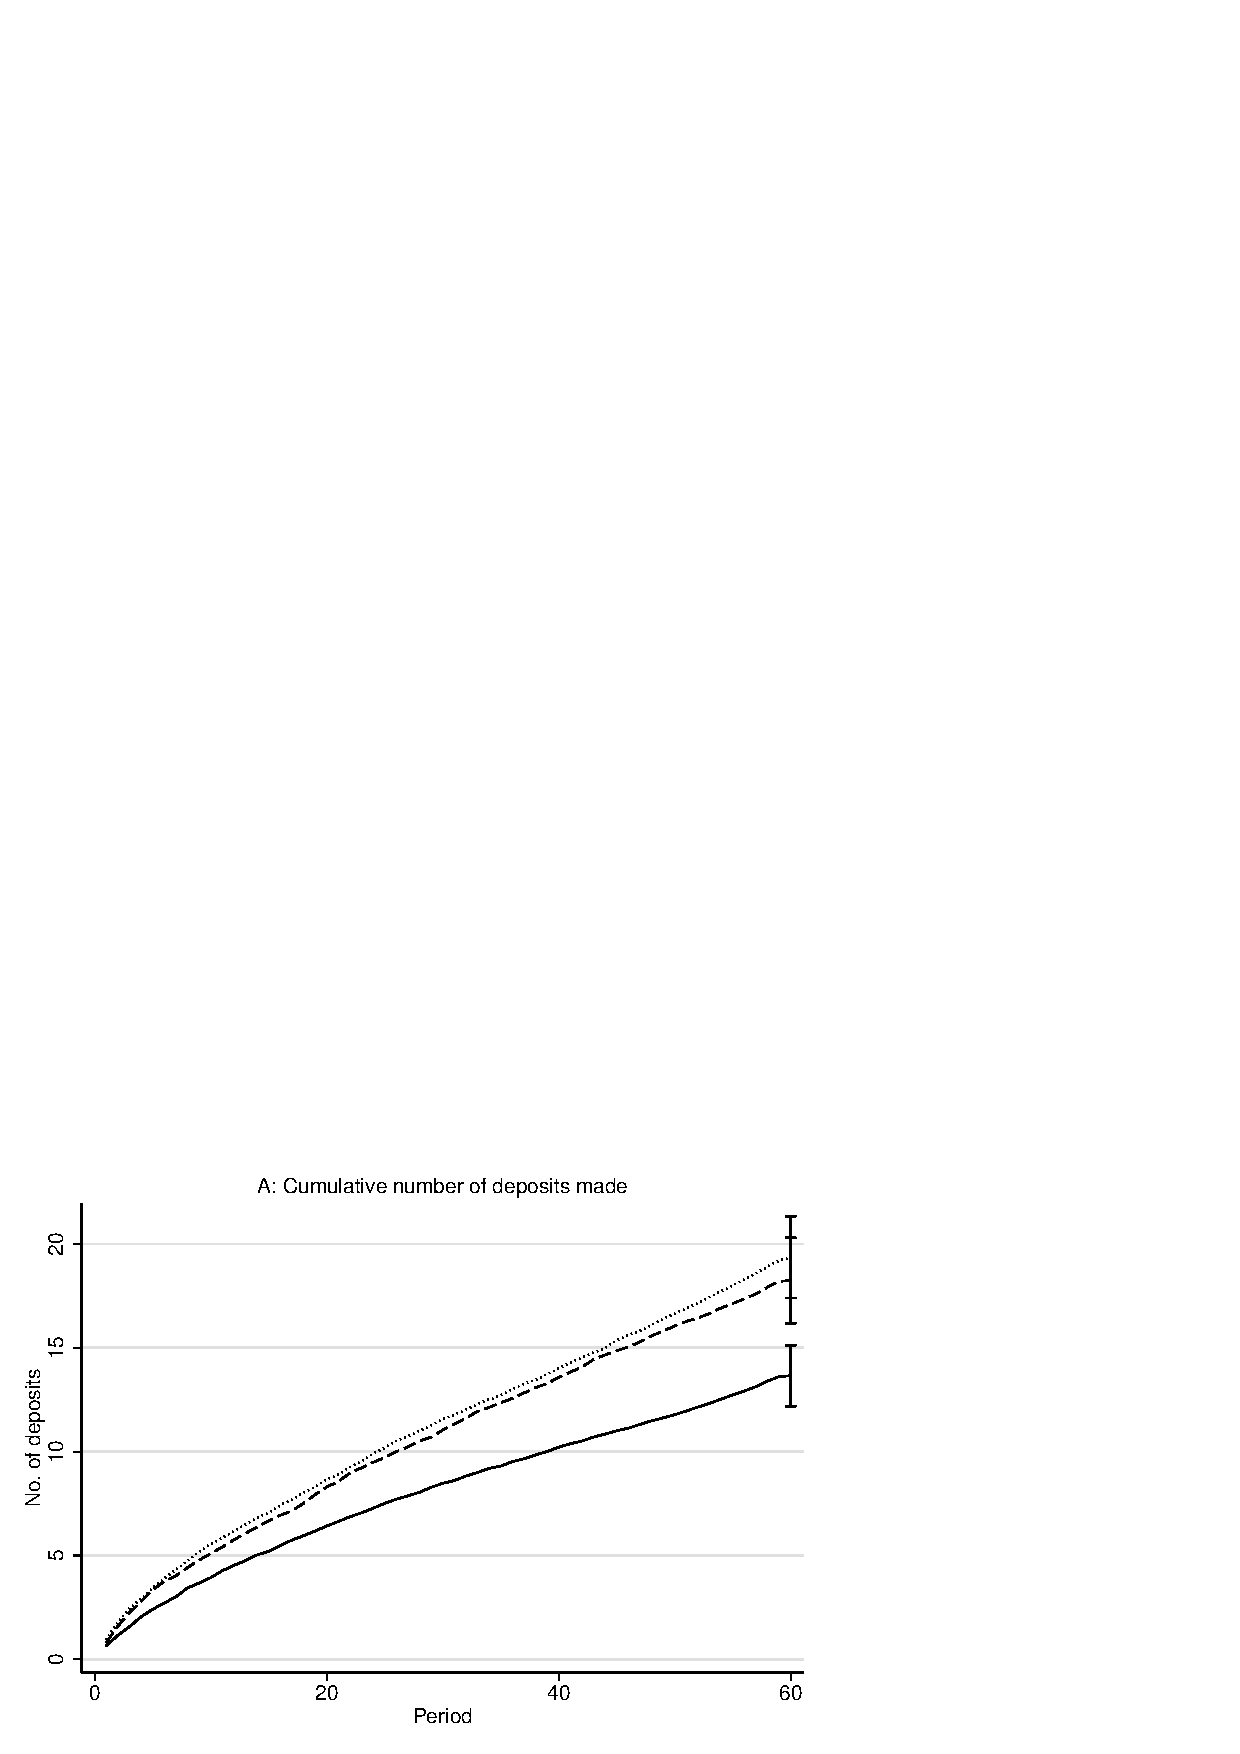
\includegraphics[height=0.8\textheight]{line-mobile_cumdeposits.pdf}
	\end{figure}

\end{frame}

\begin{frame}{Results -- Effects Over Time}

	\begin{figure}[H]
		\centering
		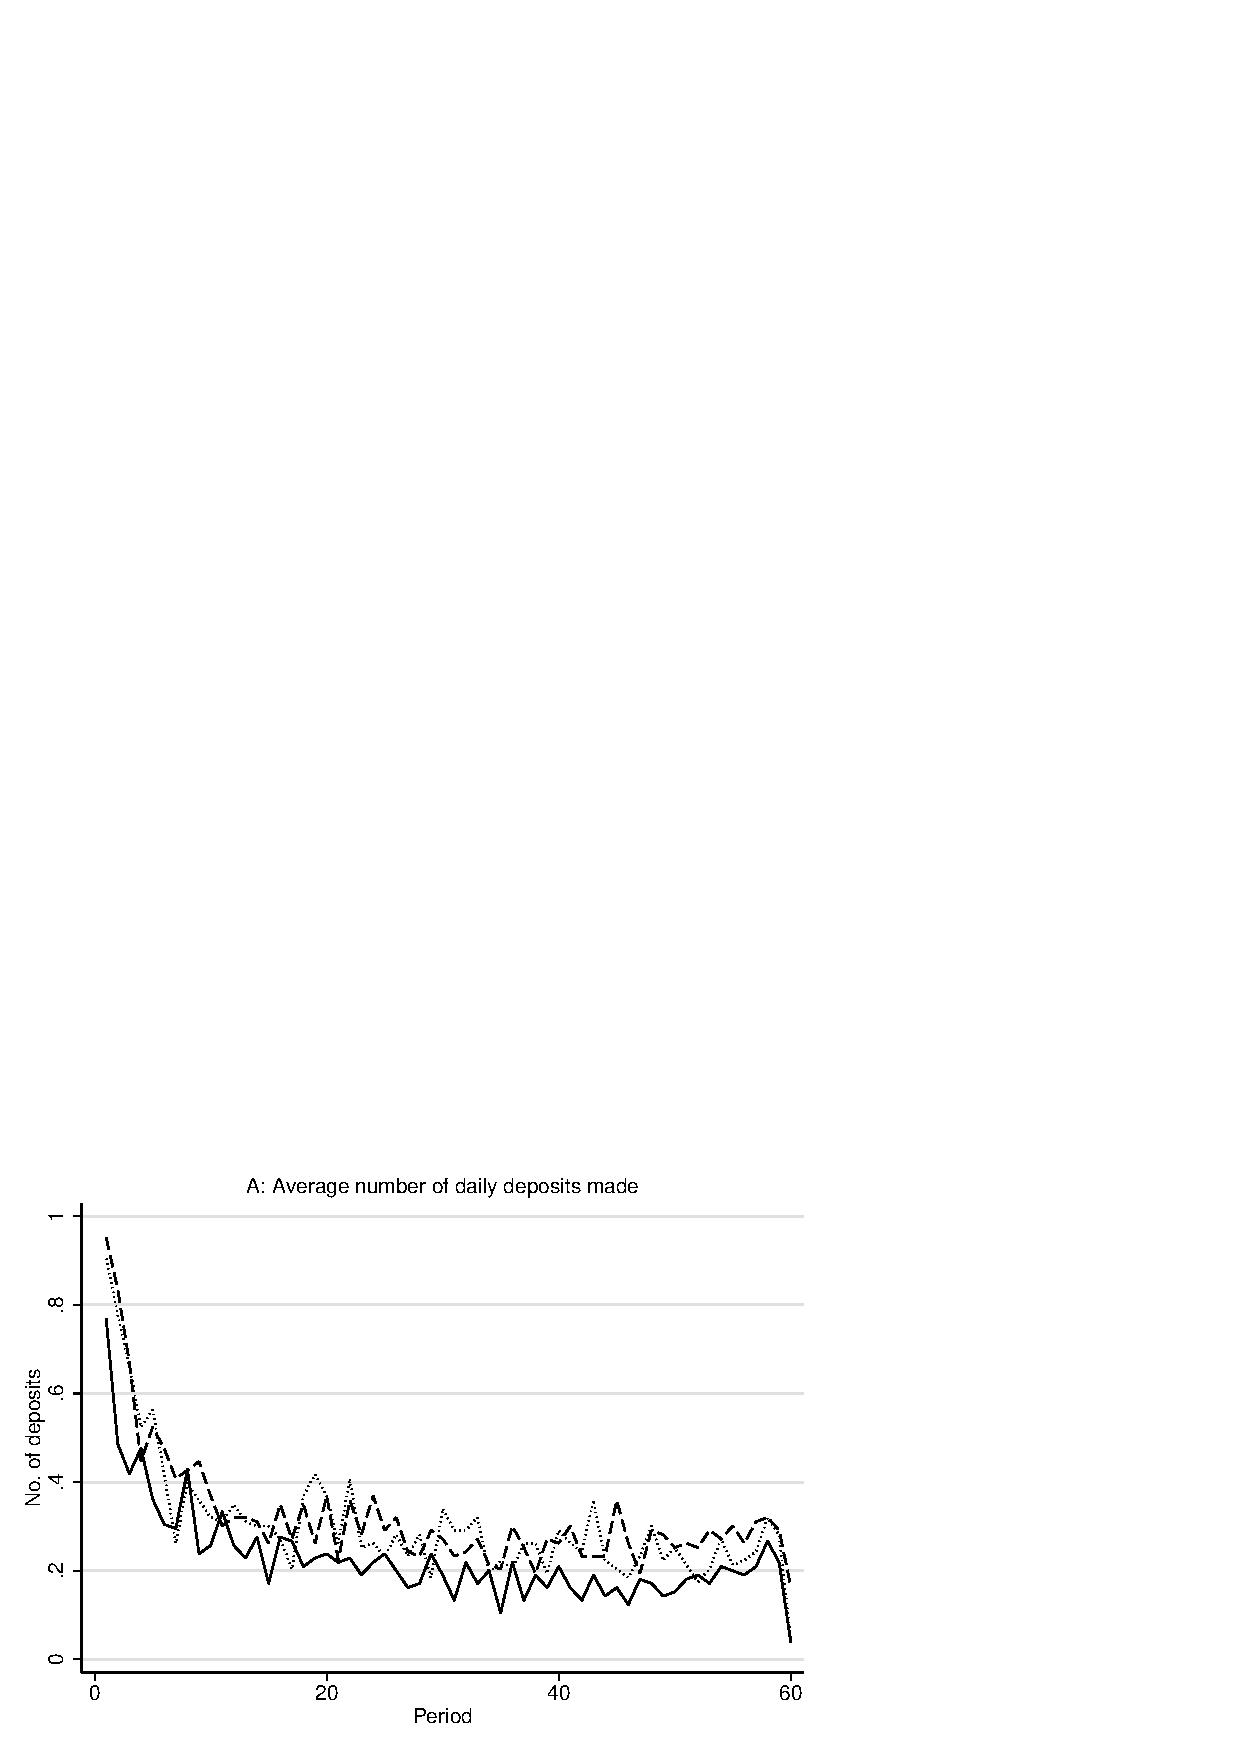
\includegraphics[height=0.8\textheight]{line-mobile_deposits.pdf}
	\end{figure}

\end{frame}

\begin{frame}{Conclusion}

	\begin{wideitemize}
		\item The savings experiment finds that:
		\begin{itemize}
			\item PLS can increase account usage but not savings per se.
			\item Behavior is consistent with regret aversion.
			\item Recently experienced regret reinforces subsequent effect.
			\item Little effect on other savings, consumption, gambling.
		\end{itemize}
		\item Further research
		\begin{itemize}
			\item Observe entire portfolio of assets, consumption.
			\item Investigate long-term effects.
			\item A structural approach to help quantify role of alternative explanations.
			\item Examine cost-effectiveness relative to other products.
			\item Understand learning and salience of regret.
			\item Understanding portfolio selection when all types of savings are available.
		\end{itemize}
	\end{wideitemize}

\end{frame}

\begin{frame}[allowframebreaks] \frametitle{References}

	\printbibliography

\end{frame}

\appendix

\begin{frame}{Regret Aversion with PLS}

	\begin{wideitemize}

		\item Suppose $u(0) = 0$ and denote $f_i$ the payoff for depositing in state $i$. 
	
		\item Saving without feedback:

		\[ \sum_{i=1}^4 p_i \cdot [u(f_i) + R(u(f_i))] \geq 0 \]

		\item Saving with feedback:	

		\[\sum_{i=1}^4 p_i \cdot [u(f_i) + R(u(f_i))] \geq \sum_{i=1}^4 p_i \cdot R(-u(f_i)) \]

		\item $R(0) = 0$ and strictly increasing implies that $R(u(f_i)) > 0$ and $R(-u(f_i)) < 0$.

		% this is incorrect

	\end{wideitemize}

\end{frame}

\begin{frame}{Demonstration}

	\begin{figure}[H]
		\centering
		\includegraphics[width=0.8\linewidth]{fig-lottery.png}
	\end{figure}

\end{frame}

\begin{frame}{Financial Inclusion}

	\begin{figure}[H]
		\centering
		\includegraphics[width=0.45\linewidth]{fig-findex.png}
	\end{figure}

\end{frame}

\begin{frame}{Lottery Draws}

	\begin{table}[htbp]\centering \def\sym#1{\ifmmode^{#1}\else\(^{#1}\)\fi} \caption{Observed and expected lottery results} \label{tab:tab-lottery} \maxsizebox*{\paperwidth}{\paperheight}{ \begin{threeparttable} \begin{tabular}{l*{3}{c}} \toprule
                    &        Freq.&         Pct. observed&      Pct. expected\\
\midrule
No match                   &        7065&       81.49&       62.43\\
One match                   &        1518&       17.51&       22.22\\
Two matches                   &          86&        0.99&       1.23\\
Complete match                   &           1&        0.01&      0.00\\
\bottomrule \end{tabular} \begin{tablenotes}[flushleft] \footnotesize \item \emph{Notes:} The first column tabulates the frequency of observed lottery ticket matches. The second and third columns report the observed and expected probabilities, respectively, of each type of lottery match. A lottery ticket was a random sequence of four numbers between 1 and 9, inclusive. Prizes were awarded according to how well a participant's lottery numbers matched the winning numbers. If the first or second numbers matched, a 10\% match of savings was awarded. If \emph{both} the first and second numbers matched, a 100\% match of savings was awarded. Finally if all numbers matched, a prize of 200 times the daily savings was awarded. \end{tablenotes} \end{threeparttable} } \end{table}


\end{frame}

\begin{frame}{Timing}

	\begin{figure}[H]
		\centering
		\includegraphics[width=0.65\linewidth]{hist-deposits.pdf}
	\end{figure}

\end{frame}

\begin{frame}{Results}{Savings}

	\begin{table}[htbp]\centering \def\sym#1{\ifmmode^{#1}\else\(^{#1}\)\fi} \caption{Treatment effects -- Self-reported savings behavior} \label{tab:reg-save} \maxsizebox*{\textwidth}{\textheight}{ \begin{threeparttable} \begin{tabular}{l*{8}{c}} \toprule
          &\multicolumn{3}{c}{No controls}&\multicolumn{3}{c}{With controls}&\multicolumn{2}{c}{Sample}\\\cmidrule(lr){2-4}\cmidrule(lr){5-7}\cmidrule(lr){8-9}
          &\multicolumn{1}{c}{(1)}&\multicolumn{1}{c}{(2)}&\multicolumn{1}{c}{(3)}&\multicolumn{1}{c}{(4)}&\multicolumn{1}{c}{(5)}&\multicolumn{1}{c}{(6)}&\multicolumn{1}{c}{(7)}&\multicolumn{1}{c}{(8)}\\
          &\multicolumn{1}{c}{Lottery}&\multicolumn{1}{c}{Regret}&\multicolumn{1}{c}{\specialcell{Difference\\\(p\)-value}}&\multicolumn{1}{c}{Lottery}&\multicolumn{1}{c}{Regret}&\multicolumn{1}{c}{\specialcell{Difference\\\(p\)-value}}&\multicolumn{1}{c}{\specialcell{Control Mean\\(SD)}}&\multicolumn{1}{c}{Obs.}\\
\midrule
Log total savings last mo.&    -0.15&    -0.05&     0.72&    -0.10&     0.12&     0.44&     3.80&      284\\
          &   (0.32)&   (0.29)&         &   (0.31)&   (0.29)&         &   (2.11)&         \\
          &   [1.00]&   [1.00]&         &   [1.00]&   [0.90]&         &         &         \\
Log M-Pesa savings last mo.&    -0.22&    -0.11&     0.70&    -0.25&    -0.17&     0.76&     1.55&      284\\
          &   (0.29)&   (0.29)&         &   (0.27)&   (0.28)&         &   (2.11)&         \\
          &   [0.70]&   [0.80]&         &   [0.70]&   [0.90]&         &         &         \\
Log ROSCA savings last mo.&     0.00&0.63$^{**}$&0.04$^{**}$&     0.05&0.64$^{**}$&0.05$^{**}$&     2.10&      283\\
          &   (0.31)&   (0.30)&         &   (0.29)&   (0.27)&         &   (2.09)&         \\
          &   [1.00]&   [0.20]&         &   [1.00]&   [0.20]&         &         &         \\
Currently saves with ROSCA&    -0.02&0.14$^{**}$&0.02$^{**}$&    -0.01&0.14$^{**}$&0.03$^{**}$&     0.54&      284\\
          &   (0.07)&   (0.07)&         &   (0.07)&   (0.06)&         &   (0.50)&         \\
          &   [1.00]&   [0.20]&         &   [1.00]&   [0.20]&         &         &         \\
\bottomrule \end{tabular} \begin{tablenotes}[flushleft] \footnotesize \item \emph{Notes:} Columns 1 - 2 report OLS estimates of the treatment effect. Columns 4 - 5 reports the estimates controlling for baseline covariates. Columns 3 and 6 report the \(p\)-values for tests of the equality of the two main treatment effects after estimation. Standard errors are in parentheses and FWER adjusted \(p\)-values are in brackets. * denotes significance at 10 pct., ** at 5 pct., and *** at 1 pct. level. \end{tablenotes} \end{threeparttable} } \end{table}

% File produced by reg-fwer.do with /Users/Justin/Repos/akiba-lottery-pub/data/clean/akiba_wide.dta on 12:41:07 17 Feb 2017 by user Justin on Stata 13.1 with seed X02be4b816237fe6e6a333726618fd6dd00043d82

\end{frame}

\begin{frame}{Results}{Savings}

	\begin{table}[h]\centering \def\sym#1{\ifmmode^{#1}\else\(^{#1}\)\fi} \caption{Treatment effects -- Expenditure} \label{tab:reg-cons} \maxsizebox*{\textwidth}{\textheight}{ \begin{threeparttable} \begin{tabular}{l*{5}{c}} \toprule
          &\multicolumn{3}{c}{Effect estimates}&\multicolumn{2}{c}{Sample}\\\cmidrule(lr){2-4}\cmidrule(lr){5-6}
          &\multicolumn{1}{c}{(1)}&\multicolumn{1}{c}{(2)}&\multicolumn{1}{c}{(3)}&\multicolumn{1}{c}{(4)}&\multicolumn{1}{c}{(5)}\\
          &\multicolumn{1}{c}{Lottery}&\multicolumn{1}{c}{Regret}&\multicolumn{1}{c}{\specialcell{Regret-\\Lottery}}&\multicolumn{1}{c}{\specialcell{Control Mean\\(SD)}}&\multicolumn{1}{c}{Obs.}\\
\midrule
Spent balance on food&     0.04&    -0.08&-0.12$^{*}$&     0.28&      284\\
          &   (0.07)&   (0.06)&   (0.06)&   (0.45)&         \\
Spent balance on school&     0.29&     0.17&    -0.13&     0.24&      284\\
          &   (0.24)&   (0.27)&   (0.32)&   (1.11)&         \\
Spent balance on business&     0.13&0.08$^{*}$&    -0.04&     0.06&      284\\
          &   (0.08)&   (0.04)&   (0.09)&   (0.25)&         \\
Spent balance on durable goods&    -0.00&    -0.03&    -0.03&     0.05&      284\\
          &   (0.03)&   (0.03)&   (0.03)&   (0.23)&         \\
Spent balance on repaying loans&     0.04&    -0.00&    -0.04&     0.11&      284\\
          &   (0.05)&   (0.04)&   (0.05)&   (0.31)&         \\
Saved balance&     0.04&     0.05&     0.01&     0.07&      284\\
          &   (0.04)&   (0.04)&   (0.05)&   (0.26)&         \\
\bottomrule \end{tabular} \begin{tablenotes}[flushleft] \footnotesize \item \emph{Notes:} Columns 1--3 report OLS estimates of the treatment effect. Standard errors are in parentheses. Columns 4--5 report the mean and SD of the control group and the number observations, respectively. Observations are at the individual level. * denotes significance at 10 pct., ** at 5 pct., and *** at 1 pct. level. \end{tablenotes} \end{threeparttable} } \end{table}

% File produced by reg-main.do with /n/homeserver2/user2a/justinra/repos/akiba-lottery-pub/data/clean/akiba_wide.dta on 00:41:46 17 Feb 2018 by user justinra on Stata 13.1 with seed X71d1d353b37e281e006fa26738e26f4500044a1c

\end{frame}

\begin{frame}{Results}{Gambling}

	\begin{table}[htbp]\centering \def\sym#1{\ifmmode^{#1}\else\(^{#1}\)\fi} \caption{Treatment effects -- Gambling behavior} \label{tab:reg-gamble} \maxsizebox*{\textwidth}{\textheight}{ \begin{threeparttable} \begin{tabular}{l*{8}{c}} \toprule
          &\multicolumn{3}{c}{No controls}&\multicolumn{3}{c}{With controls}&\multicolumn{2}{c}{Sample}\\\cmidrule(lr){2-4}\cmidrule(lr){5-7}\cmidrule(lr){8-9}
          &\multicolumn{1}{c}{(1)}&\multicolumn{1}{c}{(2)}&\multicolumn{1}{c}{(3)}&\multicolumn{1}{c}{(4)}&\multicolumn{1}{c}{(5)}&\multicolumn{1}{c}{(6)}&\multicolumn{1}{c}{(7)}&\multicolumn{1}{c}{(8)}\\
          &\multicolumn{1}{c}{Lottery}&\multicolumn{1}{c}{Regret}&\multicolumn{1}{c}{\specialcell{Difference\\\(p\)-value}}&\multicolumn{1}{c}{Lottery}&\multicolumn{1}{c}{Regret}&\multicolumn{1}{c}{\specialcell{Difference\\\(p\)-value}}&\multicolumn{1}{c}{\specialcell{Control Mean\\(SD)}}&\multicolumn{1}{c}{Obs.}\\
\midrule
Gamble more&     0.06&0.15$^{***}$&     0.16&     0.06&0.16$^{***}$&0.10$^{*}$&     0.12&      284\\
          &   (0.05)&   (0.06)&         &   (0.05)&   (0.05)&         &   (0.32)&         \\
          &   [1.00]&[0.00]$^{***}$&         &   [1.00]&[0.00]$^{***}$&         &         &         \\
Gamble less&    -0.02&     0.04&     0.24&    -0.02&     0.03&     0.33&     0.16&      284\\
          &   (0.05)&   (0.06)&         &   (0.05)&   (0.06)&         &   (0.37)&         \\
          &   [1.00]&[0.00]$^{***}$&         &   [1.00]&   [1.00]&         &         &         \\
More tempted to gamble&     0.09&     0.05&     0.56&     0.05&     0.03&     0.74&     0.47&      284\\
          &   (0.07)&   (0.07)&         &   (0.07)&   (0.07)&         &   (0.50)&         \\
          &[0.00]$^{***}$&[0.00]$^{***}$&         &   [1.00]&   [1.00]&         &         &         \\
Less tempted to gamble&    -0.01&     0.03&     0.27&    -0.00&     0.04&     0.30&     0.06&      284\\
          &   (0.03)&   (0.04)&         &   (0.03)&   (0.04)&         &   (0.25)&         \\
          &   [1.00]&[0.00]$^{***}$&         &   [1.00]&   [1.00]&         &         &         \\
\bottomrule \end{tabular} \begin{tablenotes}[flushleft] \footnotesize \item \emph{Notes:} Columns 1 - 2 report OLS estimates of the treatment effect. Columns 4 - 5 reports the estimates controlling for baseline covariates. Columns 3 and 6 report the \(p\)-values for tests of the equality of the two treatment effects. Standard errors are in parentheses and FWER adjusted \(p\)-values are in brackets. Observations are at the individual level. * denotes significance at 10 pct., ** at 5 pct., and *** at 1 pct. level. Stars on the coefficient estimates reflect unadjusted \(p\)-values. \end{tablenotes} \end{threeparttable} } \end{table}

% File produced by reg-fwer.do with /Users/Justin/Repos/akiba-lottery-pub/data/clean/akiba_wide.dta on 14:35:53  6 Mar 2017 by user Justin on Stata 13.1 with seed Xf55105a47795965f9f1f196f7765c1d200043913

\end{frame}

\end{document}

% Notes from 3/13 presentation to graduate students

% What is the most we can say about welfare since the there is a policy focus? There can be an argument made (Gertler et al., Schaner) that habit formation might be a channel. Because it depends on choice architecture, may have to accept that welfare effects are ambiguous. See aer.103.3.387 for a discussion. Given how cheap this is to implement it might be cost-effective.

% x Better explain the insurance product (at least in the presentation)

% x What are other ways subjects could have saved during the time of the study? (esp. mobile credit/savings)? M-Shwari allows people to save using MPESA since 2012. Lockbox account paying an interest of 2-5 percent earned daily for one to six months. Also provides short term credit. Half of all M-Shwari customers do not have any other bank account. In our sample, 31% of subjects use this product. There are no treatment effects on M-Shwari usage. Our product is quite similar to M-Shwari (add as footnote). https://www.cgap.org/sites/default/files/Forum-How-M-Shwari-Works-Apr-2015.pdf

% x The savings variable is a stock so say account balance. Have to check the Z-Tree because maybe this is a flow variable.

% x Explain why we use a lockbox account and explain how we might expect this to affect results/generalizability. Don't assume people are aware of this feature. (Ashraf, Dupas, Aker). This is a common feature of savings products in LIMAC. We chose it because of its ubiquity and demonstrated demand. Why do people value illiquid? Present bias with sophistication, kinship taxes, etc.

% For generalizability: explain where and whether we think this product could work

% Examine the initial dropoff in the plot: is this compositional (extensive margin) or at the intensive margin?
